\documentclass{whutmod}
\usepackage[linesnumbered,ruled,lined]{algorithm2e}
\bibliographystyle{unsrt}
\team{10}
\membera{刘子川}
\joba{编程}
\memberb{程宇}
\jobb{建模}
\memberc{祁成}
\jobc{写作}
\hypersetup{
	colorlinks=true,
	linkcolor=black,citecolor=black
}


\newcommand{\upcite}[1]{\textsuperscript{\cite{#1}}}
%%%%%%%%%%%%%%%%%%%%%%%%%%%%%%%%%题目%%%%%%%%%%%%%%%%%%%%%%%%%%%%%%%%%%%%
\title{基于动态SEIR模型的新冠疫情预测与分析}
\tihao{4} 
\everymath{\displaystyle} 
\begin{document}

	\maketitle
	\thispagestyle{empty}
%%%%%%%%%%%%%%%%%%%%%%%%%%%%%%%%%摘要%%%%%%%%%%%%%%%%%%%%%%%%%%%%%%%%%%%%
	\begin{abstract}
		本文建立了动态DSEIR传染病动力学模型并采用免疫差分进化算法,分析了具体措施对疫情传播的影响;为考察股价市场与疫情指标的相关关系,收集Bob Stock股价数据并通过SMO-SVR模型进行股价预测。
		\vspace{7pt}	%空格


		针对问题一,建立动态\textbf{DSEIR模型}并使用\textbf{免疫差分进化算法}估计模型参数,最后调整模型参数以分析卫生措施效果。本节首先根据新冠病毒疫情的\textbf{时滞特点}改进传统的SEIR模型求出预测病例人数。并通过\textbf{免疫差分进化算法}拟合预测结果与实际统计数据,估计未统计模型参数。根据美国实施居家令和提前或延后湖北省采用的严格隔离措施调整模型参数,分析预测结果的变化规律。可得出 —— 提前采取严格隔离将大幅度降湖北省低疫情损失,反之将大幅度提高损失;若即时实施居家令将大幅度降低美国疫情损失。
		\vspace{7pt}	%空格
		

	
	 针对问题二,基于多维度统计数据建立\textbf{SMO-SVR模型},预测股票市场在疫情下的变化趋势。首先以发病人数、死亡人数、治愈人数以及股市的平滑值作为决策变量对股价建立\textbf{支持向量回归}模型(SVR)进行预测。并采SMO算法将SVR模型中的对偶问题求解转化为K-T条件求解,预测八月份的股市走向。本文以\textbf{苹果股价}(AAPL)为例进行预测分析,可知股票价格与感染人数负相关,感染人数每增加200人,每股价格约下降10元左右。还可分析知股市衰退并不会持续太久,\textbf{约在六月初开始复苏}。最后通过均方根误差,平均相对误差以及纳什效益系数评价模型有效性。通过误差检验得到\textbf{八月预测误差为5\%},预测精度较高。
		\vspace{7pt}	%空格
		
		本文的优点为:1. 结合了新冠病毒的实际特点改进了SEIR模型,且使用免疫差分进化算法估计参数,使得预测模型更贴近于本次疫情的实际情况。 2.通过序列最小优化算法作为样本的训练算法,进而建立序列最小优化支持向量回归模型预测股市,从而减小算法复杂度,提高算法的求解速度。
		\keywords{
			时滞动力学模型\quad
			免疫差分进化算法\quad	
			支持向量回归机\quad
			序列最小优化\quad
		}
	\end{abstract}


%%%%%%%%%%%%%%%%%%%%%%%%%%%%%%%%%目录%%%%%%%%%%%%%%%%%%%%%%%%%%%%%%%%%%%%
	\thispagestyle{empty}
	\setcounter{page}{1}  
	\tableofcontents
	\newpage	%换页符
	

	
	\section{问题重述}	
		\subsection{问题背景}
	    	新型冠状病毒肺炎(Corona Virus Disease 2019,COVID-19),简称“新冠肺炎”,世界卫生组织命名为“COVID-19”,是指 2019 新型冠状病毒感染导致的肺炎。2020 年 3 月 11 日,世界卫生组织总干事谭德塞宣布,世卫组织认为当前新冠肺炎疫情可被称为全球大流行(pandemic)。目前,COVID-19 疫情仍在世界各地蔓延,已超过 1630 万人感染,65 万余人死亡,给世界各国的经济发展和人民生活带来了极大影响,甚至从一定程度上改变了人类的工作生活方式。
	
	在当前信息快速传播的社会中,在传染病传播周
	期内,人群一般都会经历“不重视-自我保护”2个阶段:
	在第一阶段,由于群众对疾病具体情况不知情, 对疫情
	的认知程度有限,对疾病传播缺乏有效的防备措施. 在
	此阶段中的疾病传播过程可认为符合基本再生数为常
	数的经典(Susceptible-Exposed-Infectious-Recovered,SEIR)
模型\upcite{1}。在第二阶段, 由于政府和群众高度重视,
	各种防治措施与资源被相继引入\upcite{2},加上对疾病传播途
	径已有较为准确的认知,人群会逐渐采取有效且科学
	的防控措施,使得基本再生数不断下降,直到其下降到
	小于1,并持续一段时间, 最终达到对疾病的根除。
	
		\begin{figure}[H]
		\centering
		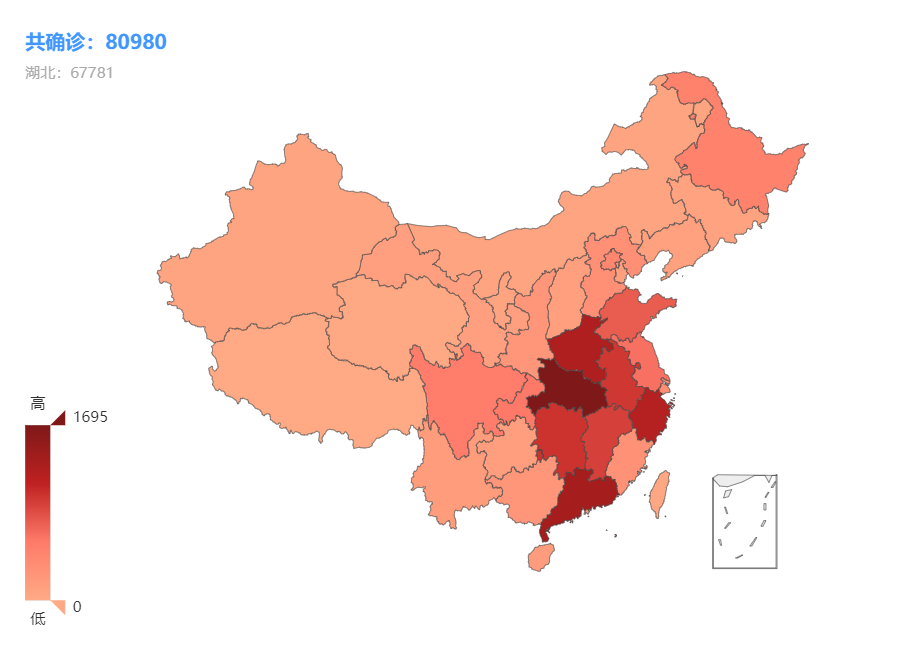
\includegraphics[width=\textwidth]{figures/demo.png}
		\caption{新型冠状病毒肺炎在中国蔓延情况}\label{lsssct}
	\end{figure}

		\subsection{问题概述}
		    围绕相关附件和条件要求,定量地研究传染病的传播规律,利用所给(不限于)资料和数据,作出预测并给出控制传染病蔓延的对策建议,具体要求如下:
				 
			
			\textbf{问题一:}建立模型,预测不同国家或地区(至少预测两个国家或地区)确诊病例和死亡病例数的变化。
			
			\textbf{问题二:}收集 COVID-19 对经济某个方面影响的数据(须说明数据获取方式或来源),建立相应的数学模型并进行预测。
			
			\textbf{问题三:}结合你们模型和预测数据,给相关国家或地区的卫生部门写一篇短文,对该国或该地区的疾病防控给出对策建议。

	
	\section{模型假设}
\begin{itemize}                                             
	\item [(1)] 假设所有感染者与潜伏者分别具有相同的疾病传播能力,且感染者的传染能量强于潜伏者。
	\item [(2)]假设实施严格的隔离措施与实施居家令分别能有效的提高隔离比例和降低人与之间的接触次数。
	\item [(3)] 假设所有康复者具有病毒抗体,不会出现二次感染的情况。
	\item [(4)] 假设股票数据真实可靠,并且所选公司能反映国家的经济情况。
\end{itemize}


	\section{符号说明}
\begin{table}[H]
	\centering
	\setlength{\tabcolsep}{12mm}
	\begin{tabular}{cc}
		\toprule[1.5pt]
		\multicolumn{1}{m{5cm}}{\centering 符号} & \multicolumn{1}{m{5cm}}{\centering 说明} \\
		\midrule[1pt]		
		$S$& 易感者的累计总数\\
		$E$&潜伏者的累计总数\\
		$I$&感染者的累计总数\\
		$S_q$&隔离易感者的累计总数\\
		$E_q$&隔离潜伏者的累计总数\\
		$H$&住院患者的累计总数\\
		$\alpha$&有效接触率\\
		$\beta$&传染率\\
		$\rho$&有效接触系数\\
		$d$&病死率\\
		\bottomrule[1.5pt]
	\end{tabular}
	\begin{tablenotes}
		\item 注:表中未说明的符号以首次出现处为准
	\end{tablenotes}
\end{table}


	\section{问题一模型的建立与求解}
		\subsection{问题描述与分析}
			问题一要求建立至少两个地区的确诊病例数与死亡数的预测模型,并基于模型对这些地区的卫生部门所采取的措施做出评论。收集整理文献可知\upcite{2,3},灰度预测、时间序列等完全基于数据的预测模型难以更改环境参数,即难以得出卫生部门采取措施对疫情数据的影响。故本节使用可灵活调整参数的动力学模型预测确诊病例数与死亡数的变化趋势。
			
			本文改进了动力学模型中的SEIR模型,基于新冠病毒的特点,添加无症状感染者元素,且使得潜伏者具有传染特性,下文称其为时滞动力学模型(DSEIR)。即总方程组中包含易感者、隔离易感者、潜伏者、隔离潜伏者、感染者以及隔离感染者与无症状感染者等变量。针对方程中的未统计参数,如接触感染率与潜伏者数量等参数,本文使用免疫差分进化算法拟合预测曲线与统计数据以求解该类未知参数。
			
			用改进的动力学模型预测湖北省与美国的确诊病例数与死亡数后,我们通过修改模型参数以探讨当地卫生部门采取的措施对疫情趋势的影响。针对湖北省,我们分别提前和延后$5$天调整模型的隔离比例以分析提前或延后采取严格的隔离措施,对疫情传播所造成的影响。针对美国,我们通过调整日平均接触人数以讨论实施或取消居家令和就地避难令对疫情传播的影响。最后给予部分参数细微震荡,对整体模型进行灵敏度分析。
			
			\begin{figure}[H]
				\centering
				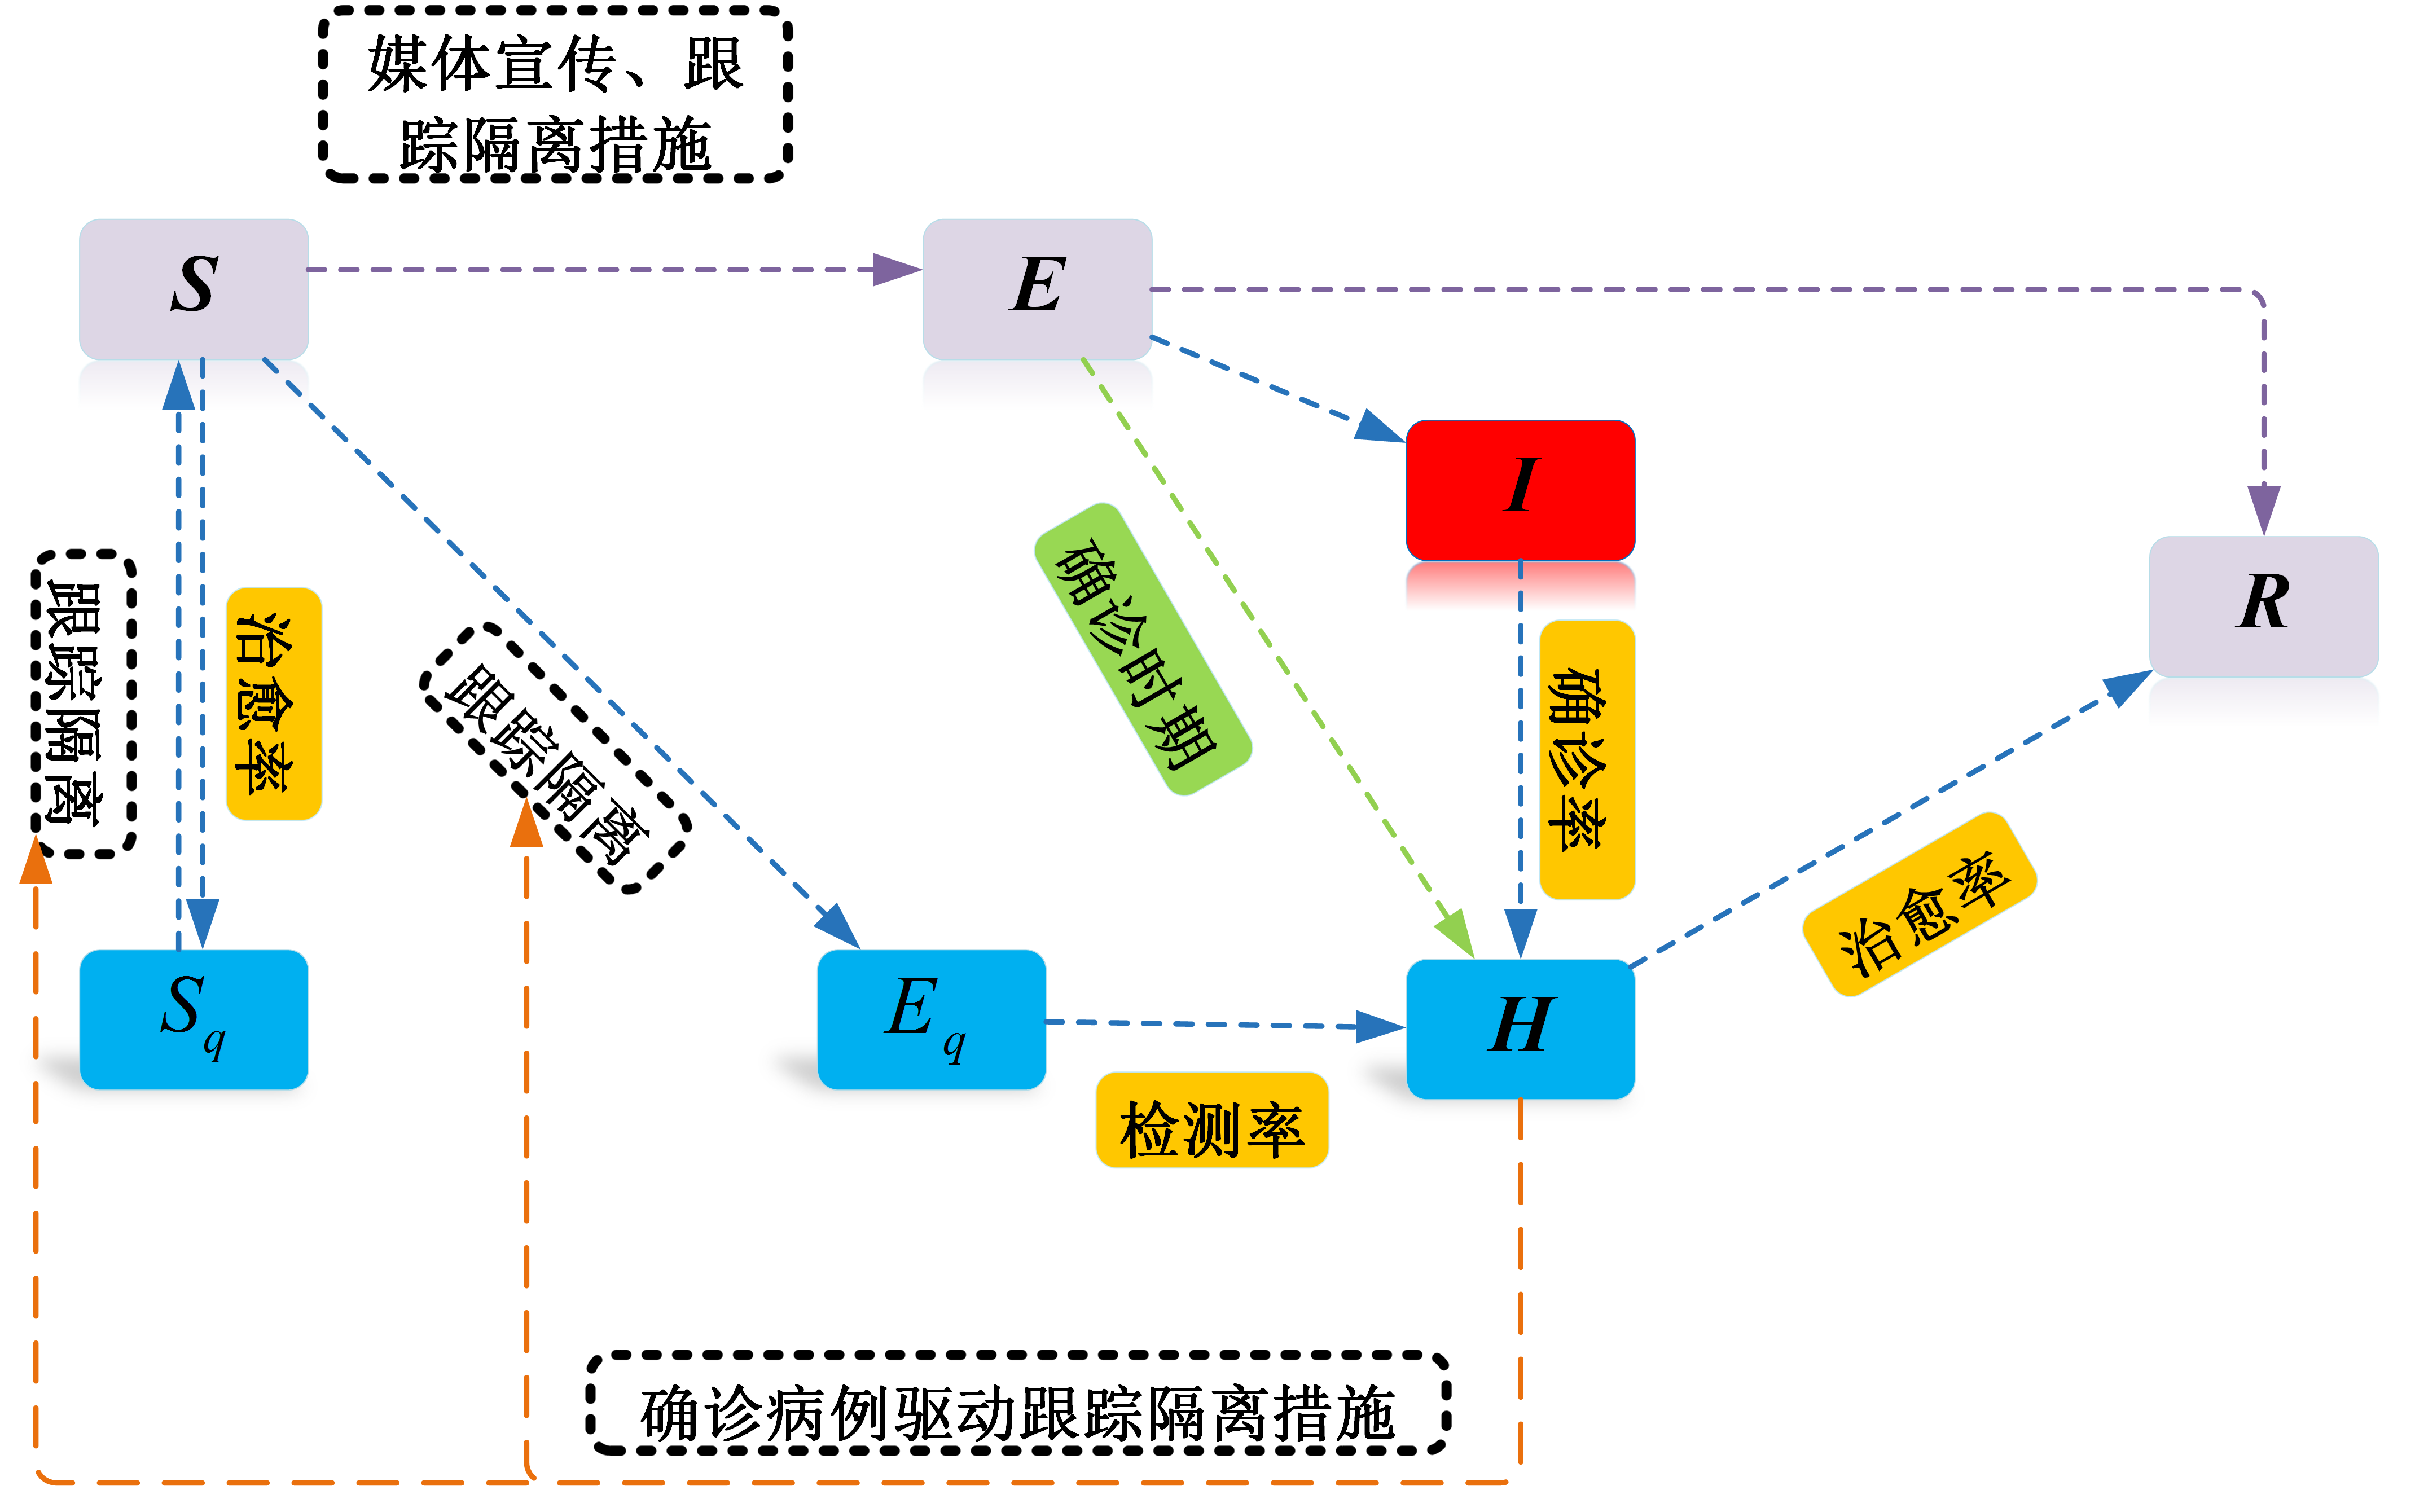
\includegraphics[width=\textwidth]{figures/kkkk.png}
				\caption{问题一人群转化关系图}\label{lct}
			\end{figure}
			
		\subsection{传染病动力学模型}
			本节介绍改进的$SEIR$模型. 研究对象是感染者、潜伏者、易感者、痊愈者等,我们使用如下记号来代表每个人群的人数:
			\begin{itemize}
				\item $S(t)$:$t$时刻易感者的累计总数;
				\item $E(t)$:$t$时刻潜伏者的累计总数;
				\item $I(t)$:$t$时刻感染者的累计总数;
				\item $S_q(t)$:$t$时刻隔离易感者的累计总数;
				\item $E_q(t)$:$t$时刻隔离潜伏者的累计总数;
				\item $H(t)$:$t$时刻住院患者的累计总数;
				\item $R(t)$:$t$时刻痊愈者的累计总数。
			\end{itemize}
		该基于人群模型有以下前提:
		
		1.潜伏者在出现明显症状前会经历$7$天的潜伏期, 一旦出现症状,潜伏者将寻求治疗,从而转为确诊的感染者;
		
		2.由于政府干预控制措施,部分感染者在潜伏期内尚未出现症状已被隔离,成为隔离潜伏者,在被隔离了平均$14$天后出现症状,成为确诊的感染者。
		
		3.模型求解过程中不考虑迁入迁出的影响,满足总人群数守恒,即
		\begin{gather*}
		\frac{\mathrm{d} S}{\mathrm{d} t}+\frac{\mathrm{d} E}{\mathrm{d} t}+\frac{\mathrm{d} I}{\mathrm{d} t}+\frac{\mathrm{d} H}{\mathrm{d} t}+\frac{\mathrm{d} E_q}{\mathrm{d} t}+\frac{\mathrm{d} S_q}{\mathrm{d} t}=0.
		\end{gather*}
		可建立模型如下:
		
		定义接触率$\alpha$、传染率$\beta$和有效接触系数$\rho$。分析可知,有效接触系数$\rho=S/(S+E+I+H)$是易感人群在随机均匀混合人群中的占比。记单个感染者个体$I_j$在$\Delta t$时间内接触和传染均匀混合个体分别为事件$A$和事件$B$。单个感染者个体$I_j$在$\Delta t$时间内接触的均匀混合个体数记为$\alpha=P(A)$,即有效接触率。将传染率定义为单个感染者个体在接触易感者的条件下传染给该易感人群的条件概率,记为$\beta=P(B|A)$。由条件概率公式,$\alpha \cdot \beta=P(A)\cdot P(B|A)=P(AB)$是单个感染者个体接触并感染易感者的概率,称为有效感染概率。
		
		分析可知易感者$S$有三种转化途径:向隔离易感者$S_q$、隔离潜伏者$E_q$和潜伏者$E$的转化速率(单位时间$\Delta t$内,转化数量$\Delta n$与同类群体的个数$n$的比值)分别为$\rho (1-\beta)q$,$ \rho \beta q$和$\rho \beta(1-q)$。此外,确认隔离期$t_d$无症状后,隔离易感者$S_q$也可向易感者$S$以$\lambda S_{q}$的速率转化。由以上分析可建立易感者$S$转化方程:
		
			\begin{gather}
			\frac{\mathrm{d} S}{\mathrm{d} t}=-\alpha\rho [\beta +q(1-\beta)]S(I+\theta E)+\lambda S_{q},
			\end{gather}
			其中,$\theta $是潜伏者相对于感染者传播能力的比值。$\lambda=1/14$是隔离解除速率,数值取隔离期的倒数。
		
			潜伏者可以向感染者转化,易感者可向潜伏者转化,可列出潜伏者$S$的转化方程:
			\begin{gather}
			\frac{\mathrm{d} E}{\mathrm{d} t}=\alpha\rho\beta(1-q) (I+\theta E)-\sigma E,
			\end{gather}
			其中,$\sigma$为潜伏者向感染者的转化速率。
			
			潜伏者可以转化为感染者,感染者的流向有死亡、被治愈和被隔离。定义病死率$d$、感染者恢复率$\varsigma_I$和隔离速率$\sigma_I$,对感染者有:
			\begin{gather}
			\frac{\mathrm{d} I}{\mathrm{d} t}=\sigma E-(\sigma_I+d+\varsigma_I)I.
			\end{gather}
			
			对于被隔离的群体,隔离易感者$S_q$与易感者相互转化;隔离潜伏者$E_q$来源于易感者,可转化为隔离感染者。定义$\delta_q$是隔离潜伏者向隔离感染者的转化速率,则有
			\begin{gather}
			\frac{\mathrm{d} S_q}{\mathrm{d} t}=\alpha\rho q(1-\beta)(I+\theta E)-\lambda S_q,
			\end{gather}
			\begin{gather}
			\frac{\mathrm{d} E_q}{\mathrm{d} t}=\rho \alpha \beta q(I+\theta E)-\delta_q E_q.
			\end{gather}
			
			对住院患者,感染者和隔离的潜伏者向住院患者的转化速率分别是$\delta_I$和$\delta_q$,住院患者流向为死亡和康复,对应系数为死亡率$d$和住院患者恢复率$\varsigma_H$。
			\begin{gather}
			\frac{\mathrm{d}H }{\mathrm{d} t}=\delta_I I+ \delta_q E_q-(d+\varsigma_H )H.
			\end{gather}
			
			对死亡病例,有
			\begin{gather}
			\frac{\mathrm{d} D}{\mathrm{d} t}= D + d(H+I).
			\end{gather}
			
			最后,痊愈者来源有感染者和住院患者,故对痊愈者有
			\begin{gather}
			\frac{\mathrm{d} R}{\mathrm{d} t}=\varsigma_I I+\varsigma_H H.
			\end{gather}
			
			模型的总表达为:
			\begin{spacing}{2}
			\begin{gather}
			\left\{\begin{array}{l}
			\frac{\mathrm{d} S}{\mathrm{d} t}=-\alpha\rho [\beta +q(1-\beta)]S(I+\theta E)+\lambda S_{q},
			\\ \frac{\mathrm{d} E}{\mathrm{d} t}=\alpha\rho\beta(1-q) (I+\theta E)-\sigma E,
			\\ \frac{\mathrm{d} I}{\mathrm{d} t}=\sigma E-(\sigma_I+d+\varsigma_I)I,
			\\ \frac{\mathrm{d} S_q}{\mathrm{d} t}=\alpha\rho q(1-\beta)(I+\theta E)-\lambda S_q,
			\\ \frac{\mathrm{d} E_q}{\mathrm{d} t}=\rho \alpha \beta q(I+\theta E)-\delta_q E_q,
			\\ \frac{\mathrm{d}H }{\mathrm{d} t}=\delta_I I+ \delta_q E_q-(d+\varsigma_H )H,
			\\ \frac{\mathrm{d} R}{\mathrm{d} t}=\varsigma_I I+\varsigma_H H,
			\\\frac{\mathrm{d} D}{\mathrm{d} t}= D + d(H+I).
			\end{array}\right.
			\end{gather}
			\end{spacing}
		\subsection{免疫差分进化算法}
		%\paragraph{初始化}
		本文设计免疫差分进化算法估计微分方程组中的未知参数,定义决策向量为
		\begin{gather}
		X=[x_1,x_2,x_3,x_4],
		\end{gather}
		其中$x_1$、$x_2$、$x_3$和$x_4$分别表示每个患者的日平均接触人数、接触感染概率、初始潜伏者数量以及潜伏者相对于感染者传播能力的比值。将目标函数定义为损失函数如下
		\begin{gather}
		min Loss(X)=\sum_{t=1}^T (|\frac{D_r(t)-D(t)}{D_r(t)}|+|\frac{R_r(t)-R(t)}{R_r(t)}|+|\frac{H_r(t)-H(t)}{H_r(t)}|),
		\end{gather}
		其中$T$表示选取数据的终止节点,即表示选取用于估计参数的数据来自疫情发生的第$1$天到第$T$天。$D_r(t)$、$R_r(t)$与$H_r(t)$分别表示疫情发生后第$t$天的死亡人数、治愈人数和医院患者人数的真实数据;$D(t)$、$R(t)$与$H(t)$分别表示其对应的由SEIR模型。损失函数$Loss$表示预测结果与实际结果间的距离,即$Loss$值越小,预测曲线就与真实曲线越接近。
		\paragraph{种群初始化}
		在解空间中随机产$p$个初始个体$
		X_i(0)=[x_1,x_2,x_3,x_4],(i=1,2,3,\cdots,p).
		$
		其中第$i$个个体的第$j$维取值方式如下
		\begin{gather*}
		x_{i,j}(0)=x_{j,min}+rand(0,1)(x_{j,max}-x_{j,min}),\\i=1,2,3,\cdots,p,j=1,2,3,4,
		\end{gather*}
		其中$p$表示种群规模,$x_{j,max}$和$x_{j,min}$分别表示决策变量$X$第$j$维的
		取值范围上界与下界。
		\paragraph{变异}
		在第$g$次迭代中,生成变异个体$H_i(g)$,从种群中随机选取三个个体$X_{p1}(g)$,$X_{p2}(g)$和$X_{p3}(g)$,且$p_1\neq p_2\neq p_3\neq i$,生成的变异向量为
	    \begin{gather*}
	    H_i(g)=X_{p1}(g)+F(g)*(X_{p2}(g)-X_{p3}(g)),
	    \end{gather*}
	    $F(g)\in (0,1)$是每一代中的放缩因子,其服从柯西分部如下
	    \begin{gather*}
	    F(g)=cauchyrnd(uF,0.1),
	    \end{gather*}
	   其中$uF$是$F$的期望值,本文取值为$uF=0.5$。
		\paragraph{交叉}
		对第$g$代种群中第$i$个体进行交叉操作,生成交叉个体$V_i(g)$,具体表达式如下:
		\begin{gather}
		v_{i,j}=\left\{\begin{matrix}h_{i,j}(g),rand(0,1)\leq cr_{i},
		\\ x_{i,j}(g),rand(0,1)>cr_{i},
		\end{matrix}\right.
		\end{gather}
     	其中$cr_{i}\in[0.1,0.6]$是个体$i$的交叉概率,参数$cr_{i}$将进行自适应调整,具体表达式如下:
		\begin{gather}
		cr_{i}=\left\{\begin{matrix}cr_{l}+(cr_{u}-cr_{l})\frac{Loss_{i}-Loss_{min}}{Loss_{max}-Loss_{min}} , Loss_{i}>\overline{Loss},
		\\ cr_{l},Loss_{i}\leqslant  \overline{Loss}.
		\end{matrix}\right.
		\end{gather}
	    \paragraph{免疫选择}
	    混合第$g$代的交叉个体$V(g)$与原始个体$X(g)$,得到待选组$\left \{ X '(g+1)\right \}$如下
	    \begin{gather*}
	    X_i '(g+1)=\left\{\begin{matrix}  X_i (g),i\leqslant p,
	    \\  V_{i-p} (g),i>p.
	    \end{matrix}\right.
	    \end{gather*}
	    
		个体 $X_a '(g+1)$和$X_b '(g+1)$的亲和度$S_{a,b}$可表示为
		\begin{gather}
		S_{a,b}=\sqrt{\sum _{i=1}^4( \frac{x_{i,a}-x_{i,b}}{x_{i,max}-x_{i,min}})^2},
		\end{gather}
		$S_{a,b}$为$X_a '(g+1)$和$X_b '(g+1)$的归一化距离,表示个体$X_a '(g+1)$和$X_b '(g+1)$的相似性。定义个体$X_i '(g+1)$的抗体浓度为$C_{i}$,即
		\begin{gather*}
		C_{i}=\frac{1}{2p}\sum _{j=1}^{2p} N_{i,j},\\
		N_{i,j}=\left\{\begin{matrix}1,S_{i,j}\geqslant \mu ,
		\\ 0,S_{i,j}< \mu ,
		\end{matrix}\right.
		\end{gather*}
		$\mu(\mu\in[0,1])$为相似度阈值,即当个体$i$和$j$的亲和度$S_{i,j}\geqslant \mu$时认为个体$i$和$j$为相似个体。$C_{i}$即为$\left \{ X '(g+1)\right \}$中$X_i '(g+1)$的相似个体所占比例,$C_{i}$越大即表示$X_i '(g+1)$所在区域的个体密度越大。我们优先将损失函数$Loss$值最优的前$\sigma$个解放入下一代个体$\left \{ X(g+1)\right \}$中以防止最优解丢失。再计算剩余个体的复合适应度函数,即个体$i$的复合适应度函数可表示为
	    \begin{gather}
	  min F(X_i '(g+1))=\frac{Loss(X_i '(g+1))-Loss_{min}}{Loss_{max}-loss_{min}}+C_{i}
		\end{gather}
		即选取复合适应度函数$F$较优的剩余$p-\sigma$个个体放入下一代个体$\left \{ X(g+1)\right \}$中。重复迭代上述算法$G$次后终止算法并输出最优参数集$X_{best}$。
	
		
        \subsection{实验结果及分析}
        本文先后采取湖北和美国的数据预测确诊病例和死亡病例数的变化。并设立在\textbf{2020年1月22日}时两地的初值统计参数如下表所示
                	\begin{table}[H]
        	\setstretch{0.8}  %设置表的行间距
        	\centering		
        	\caption{模型统计前初值参数}\label{sdsssf}
        	\begin{tabular}{cccc}
        		\toprule[2pt]
        		\multicolumn{1}{m{4cm}}{\centering 参数名称}
        		& \multicolumn{1}{m{3cm}}{\centering 湖北省}
        		& \multicolumn{1}{m{3cm}}{\centering 美国}
        		& \multicolumn{1}{m{3cm}}{\centering 来源}
        		\\
        		\midrule[1pt]
        		人口总数&  59170000& 310000000&goolge\\ 
        		感染者&   786& 3&goolge\\ 
        		尚在接受医学观察的人数&  2776& 124&参考文献\upcite{2}\\ 
        		正在被隔离的潜伏者&  400& 10&估计值\\ 
        		 正在住院的患者&  1186& 20&参考文献\upcite{2}\\ 
        		 出院人数&  31& 0&google\\ 
        		死亡人数&  3& 0&百度\\ 
        		\bottomrule[2pt]	
        	\end{tabular}
        \end{table}
        
        使用免疫差分进化算法可求得湖北省与美国的未统计参数如表~\ref{sdf}~所示,其中初始潜伏者数量的步长为25进行遍历。
        
        	\begin{table}[H]
        	\setstretch{1.5}  %设置表的行间距
        	\centering		
        	\caption{免疫差分进化算法求得的未统计参数}\label{sdf}
        	\begin{tabular}{ccc}
        		\toprule[2pt]
        		\multicolumn{1}{m{5cm}}{\centering 参数名称}
        		& \multicolumn{1}{m{4cm}}{\centering 湖北省}
        		& \multicolumn{1}{m{4cm}}{\centering 美国}
        		\\
        		\midrule[1pt]
        	日平均接触人数&   4.13& 14.28\\ 
        	接触感染概率& 0.4384	& 0.6851\\ 
        	初始潜伏者数量& 	125& 1100\\ 
        	潜伏者与患者感染能力比& 1.00&1.00\\
        		\bottomrule[2pt]	
        	\end{tabular}
		\end{table}
        
        根据该参数求得预测参数与实际统计参数可解得湖北省数据预测曲线如图~\ref{sd}~所示,其中取隔离解除速率 $\lambda =\frac{1}{14}$,潜伏者向感染者的转化速率 $\sigma=\frac{1}{7}$。取1月22日前,即严格的隔离措施执行前隔离比例$q=0.2$,取执行之后的隔离比例为$q=0.95$。
        \begin{figure}[H]
	\centering
	\subfigure{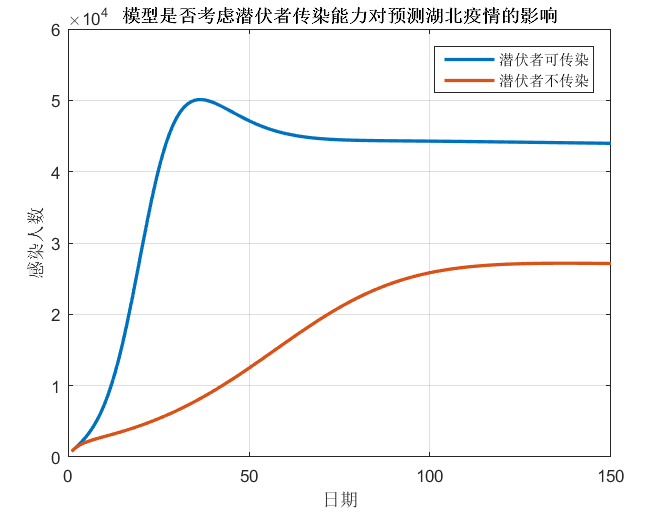
\includegraphics[height=6.5cm,width=7.5cm]{figures/untitled.png}}
	\subfigure{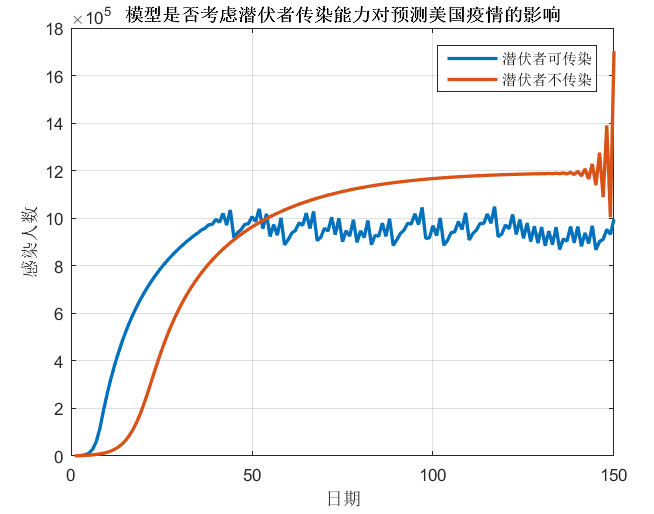
\includegraphics[height=6.5cm,width=7.5cm]{figures/untitled2.png}}
	\caption{湖北省和美国两地的感染者预测曲线}\label{sd}
\end{figure}

        若使严格隔离措施推后5日执行,即使得2月1日前隔离比例为$q=0.2$,之后的隔离比例为$q=0.99$,可得预测曲线如图~\ref{label}~所示
                \begin{figure}[H]
        	\centering
        	\subfigure[湖北推后5日执行]{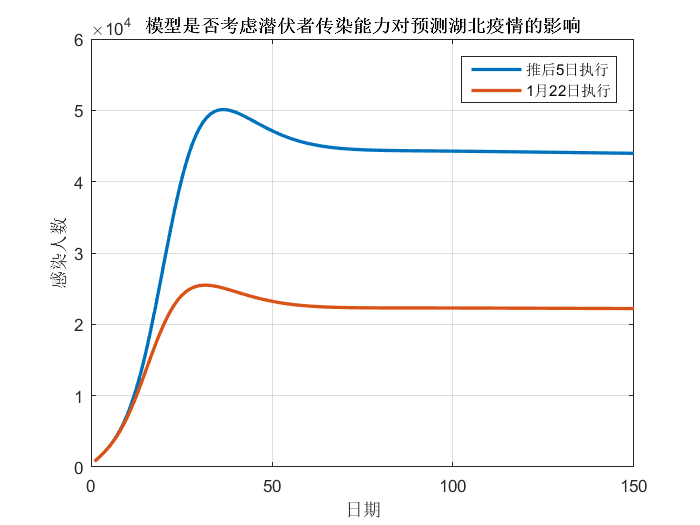
\includegraphics[height=6cm,width=7.5cm]{figures/untitled222.png}}
        	\subfigure[美国推后5日执行]{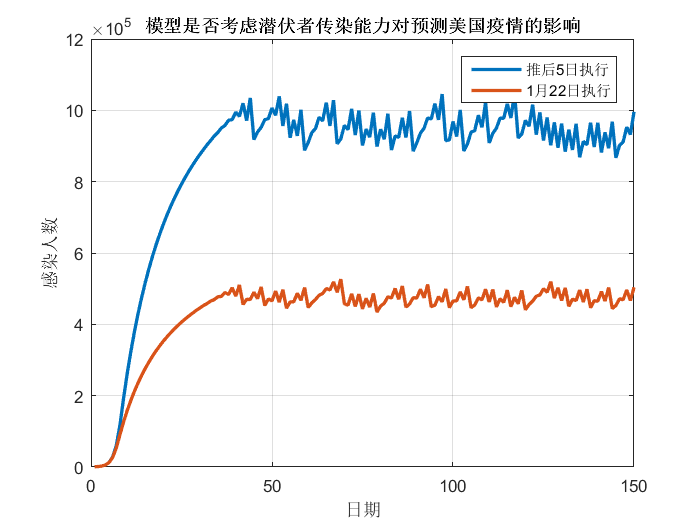
\includegraphics[height=6cm,width=7.5cm]{figures/untitle.png}}
        	\caption{湖北省和美国两地懈怠措施的感染者预测曲线}\label{label}
        \end{figure}
    
    
        由图可知,推后5日执行严格隔离措施将使得疫情高峰于\textbf{50天后}到来。最高感染人数将分别达到\textbf{5万人/120万人},是原始数据的\textbf{两倍}左右。死亡人数将达到\textbf{3千/14万人},是原始数据\textbf{的3倍}。若使严格隔离措施提前3日执行,即使得1月19日前隔离比例为$q=0.2$,之后的隔离比例为$q=0.99$,可得预测曲线如图~\ref{lasssbel}~所示
        
                        \begin{figure}[H]
        	\centering
        	\subfigure[湖北提前3日执行]{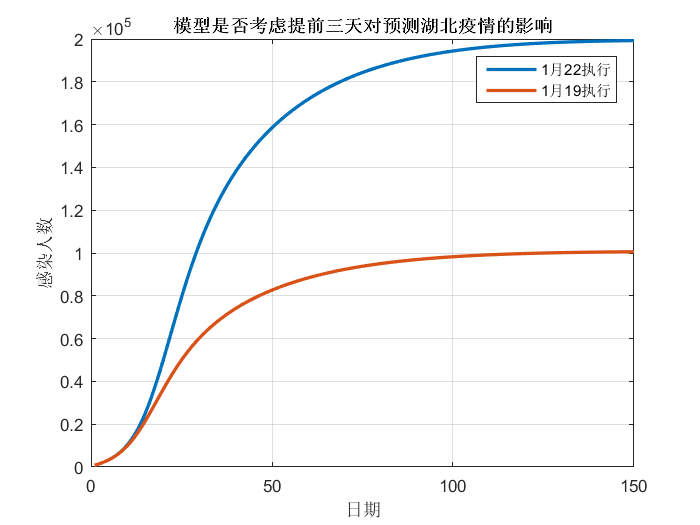
\includegraphics[height=6cm,width=7.5cm]{figures/untitled123.png}}
        	\subfigure[美国执行全美实施居家令]{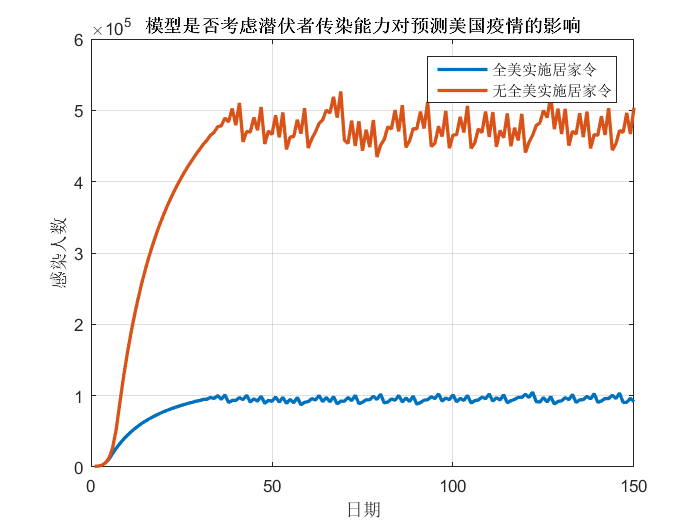
\includegraphics[height=6cm,width=7.5cm]{figures/untitld.png}}
        	\caption{湖北省和美国两地及时管控措施的感染者预测曲线}\label{lasssbel}
        \end{figure}
        
        若全美实施居家令和湖北提前3日执行,即使得日平均接触人数减半,即仅提前三天执行隔离措施将大幅度降低疫情损失,而推后5日执行隔离措施将使得疫情损失大幅度增长。取隔离比例$q=0.1$可得美国测曲线如图~\ref{lasssbel}~所示。提前3日执行严格隔离措施将使得疫情高峰于\textbf{30天后}到来。最高感染人数将分别达到\textbf{2万人/60万人},是原始数据的0.7倍。死亡人数将达到\textbf{8百/7万人},是原始数据的0.6倍。即若及时管控严格将使得疫情损失大幅度降低。
        
        	
        \subsection{灵敏度分析}
        以湖北为例,分别使得患者的日平均接触人数、接触感染概率、初始潜伏者数量以及潜伏者相对于安全措施的比值上下波动$15\%$,观察最高感染人数与死亡人数值是否发生改变。
        
        \begin{figure}[H]
        	\centering
        	\subfigure{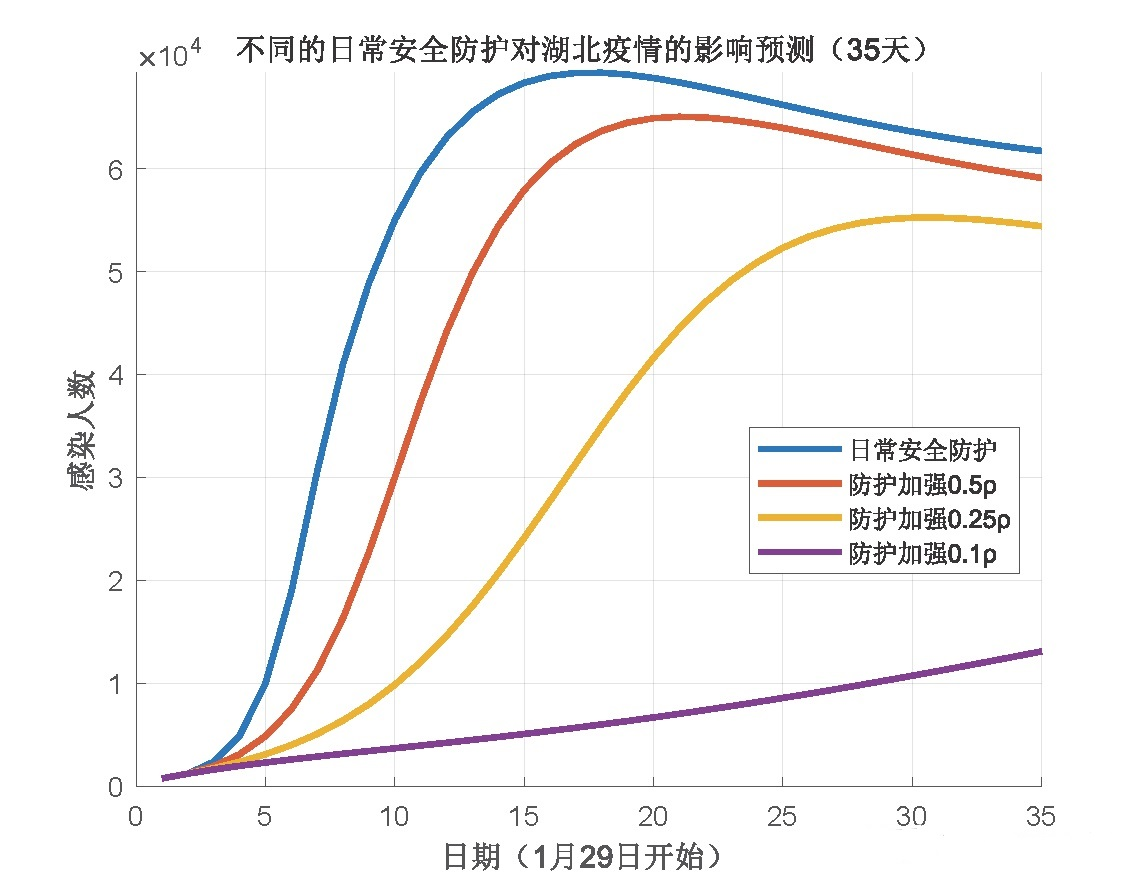
\includegraphics[height=6cm,width=7.5cm]{figures/y3.png}}
        	\subfigure{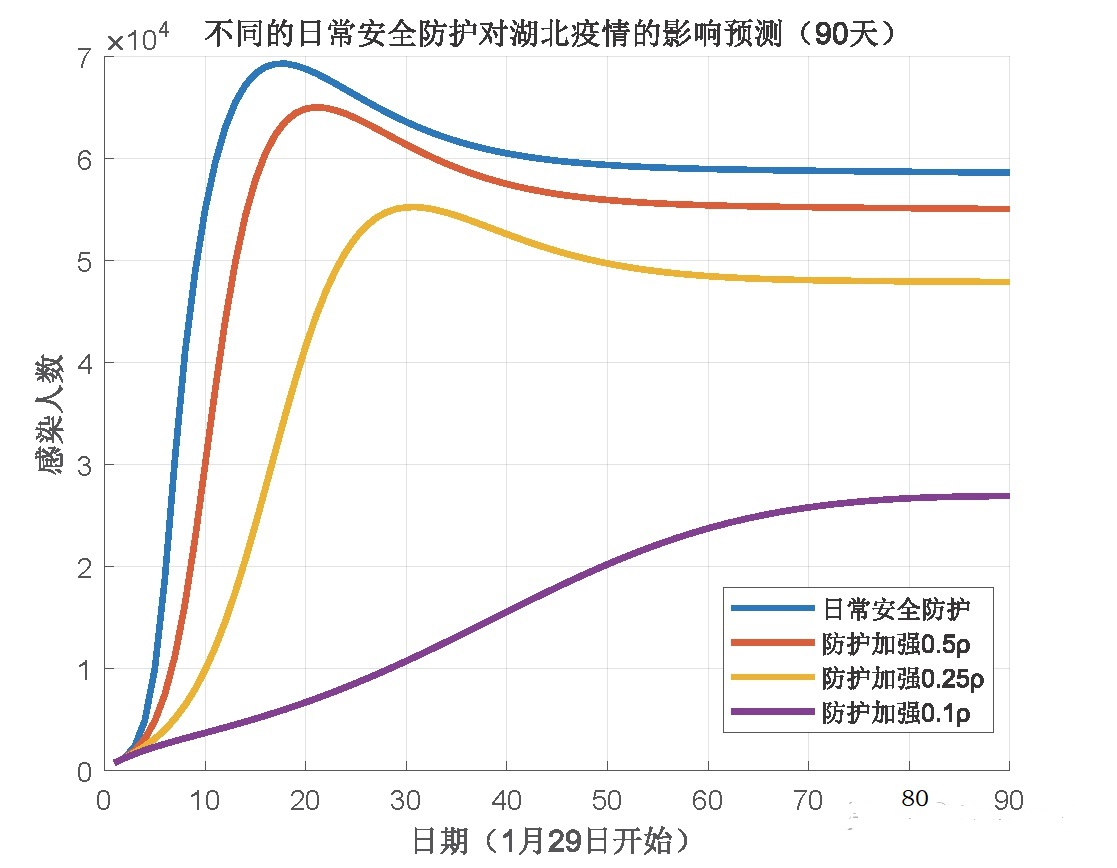
\includegraphics[height=6cm,width=7.5cm]{figures/y4.png}}
        	\caption{不同的日常安全防护对湖北的疫情影响预测}
        \end{figure}
        
        分析图~\ref{label}~可知,随着人员之间日常接触率增大,个人日常安全防护将显得尤其重要。上图分析了有效接触系数降低对疫情发展的影响(假设诊断标准未发生变化),设置人员之间接触率$c=10.15$。有效接触系数分别取0.5、0.25和0.1时。个人日常防护措施将在保障个人安全的同时,对遏制疫情的发展起到重要作用。严格的日常安全防护有助于感染人数峰值时间的提前,并且有助于峰值人数的降低。在严格个人防护措施下($\rho=0.1$),感染人数峰值可下降接近50\%。
        

       本文还模拟了追踪隔离措施,即追踪隔离比例下降对疫情发展的后果。如下图所示,当隔离比例下降为0.9、0.8和0.6倍时,感染人数的上升速率和峰值均会增加(假设诊断标准未发生变化,即感染人数未突跳)。尤其当取$0.6q$时,感染人数峰值提高约两倍。由此可见,严格的医学追踪隔离是防止疫情发展的有效手段。
          \begin{figure}[H]
        	\centering
        	\subfigure{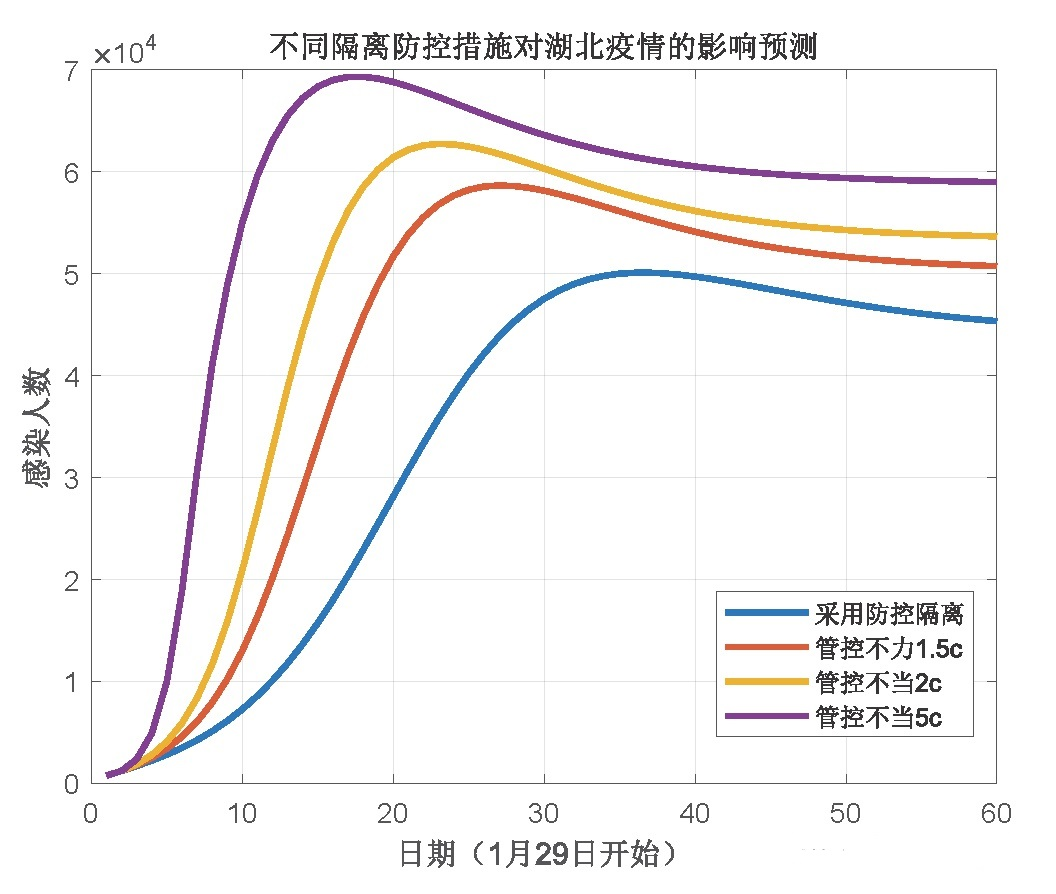
\includegraphics[height=5cm,width=7.5cm]{figures/y1.png}}
        	\subfigure{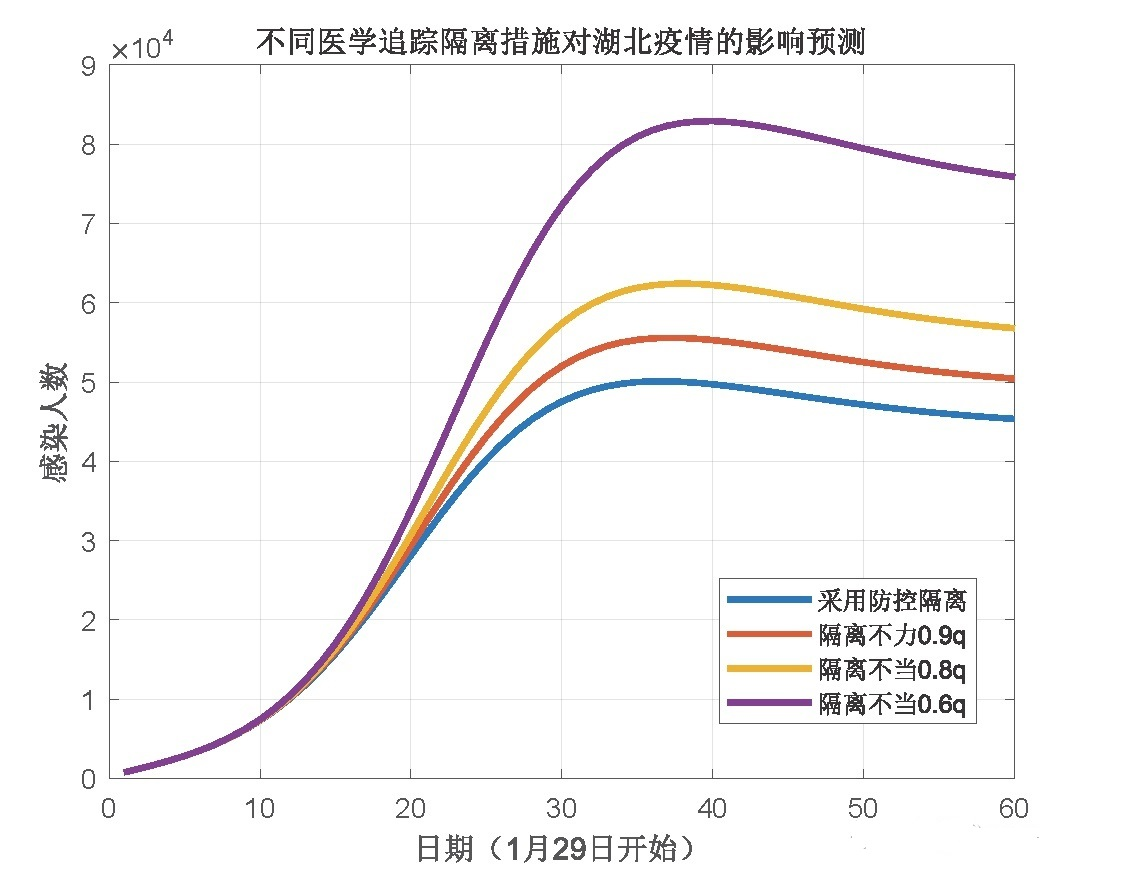
\includegraphics[height=5cm,width=7.5cm]{figures/y2.png}}
        	\caption{追踪隔离措施对湖北的疫情影响预测}
        \end{figure}
        
  
	\section{问题二模型的建立与求解}
		\subsection{问题描述与分析}
			问题二要求收集某方面经济数据并说明起影响, 资本市场是现代市场经济的重要组成部分,是实施国家发展战略、调整产业结构的重要平台和手段,本文根据2020年1月22日至7月10日的A股日历史K线数据进行预测。
			
			

    		我国股票市场较全面地反映了疫情对投资者情绪、流动性需求和实体经济产生冲击所形成的影响。今年市场A股走势如图~\ref{lssssssct}~所示。例如。 1 月 23 日当天沪深 300 指数大幅下跌,同时成交额放大。 1 月 24 日至 2 月 2 日之间是春节假期,股市没有交易,但是这一阶段全国范围内的新增感染人数不断攀升, 投资者的情绪不断累积,加之疫情已经开始冲击实体经济,所以在 2 月 3 日股市开始交易后,沪深 300 指数有一个更大幅度的下探,成交量也激增。

			\begin{figure}[H]
				\centering
				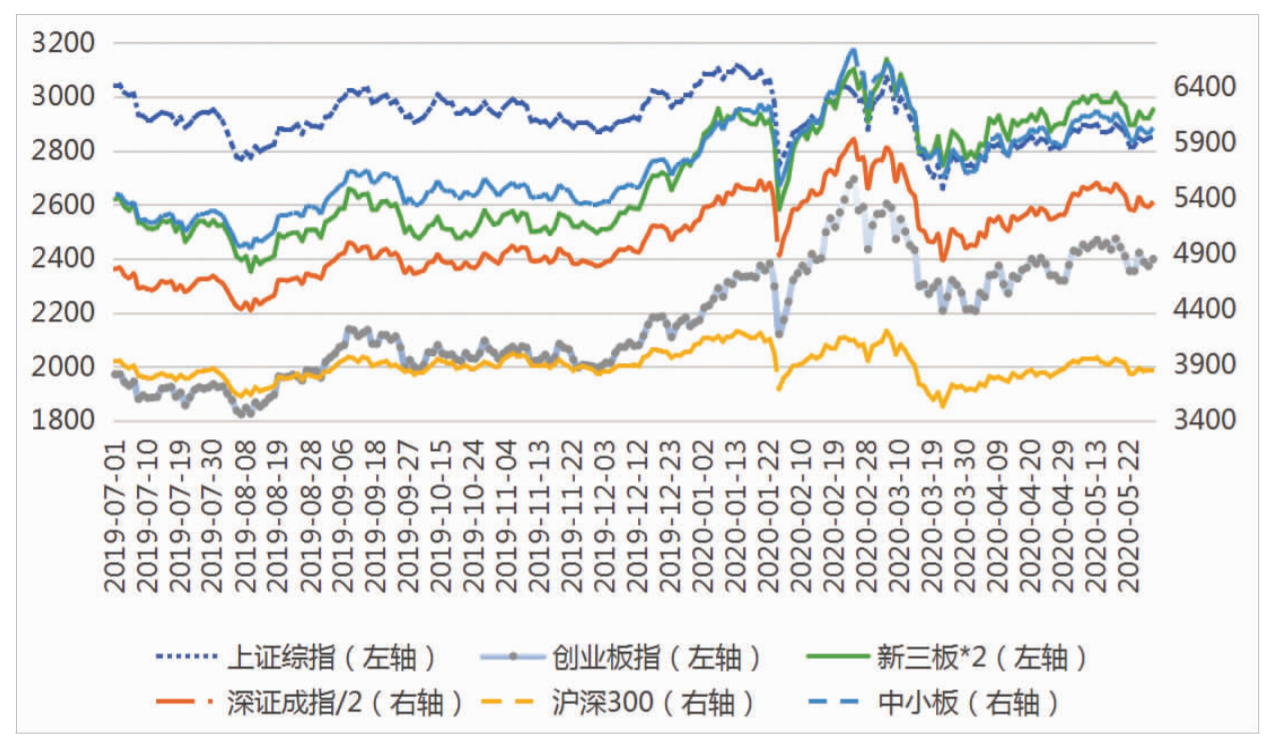
\includegraphics[width=.8\textwidth]{figures/A1.png}
				\caption{A股主要指数走势对比图}\label{lssssssct}
			\end{figure}


如图~\ref{lssssdddssct}~所示,纵观 2019 年,制造业 PMI 一直在 50 这个“荣枯线”上下浮动, 而疫情的爆发使 PMI 在 2020 年 2 月创下了一个极低值, 消费者信心指数和消费者预期指数同样降幅巨大。 东东方财富数据显示,截至 2020 年4 月 30 日,A 股 3832 家上市公司中有 3523 家披露了 2020 年一季报,A股上市公司一季度合计实现营业收入 10.59 万亿元,同比下降 7.91\%,其中主板营收增速下滑7.89\%,中小板总营收下滑 5.25\%,创业板下滑 10.82\%。由此可见,疫情对经济的影响及其巨大,为此本节采用大盘股市的数据进行预测。

		\begin{figure}[H]
	\centering
	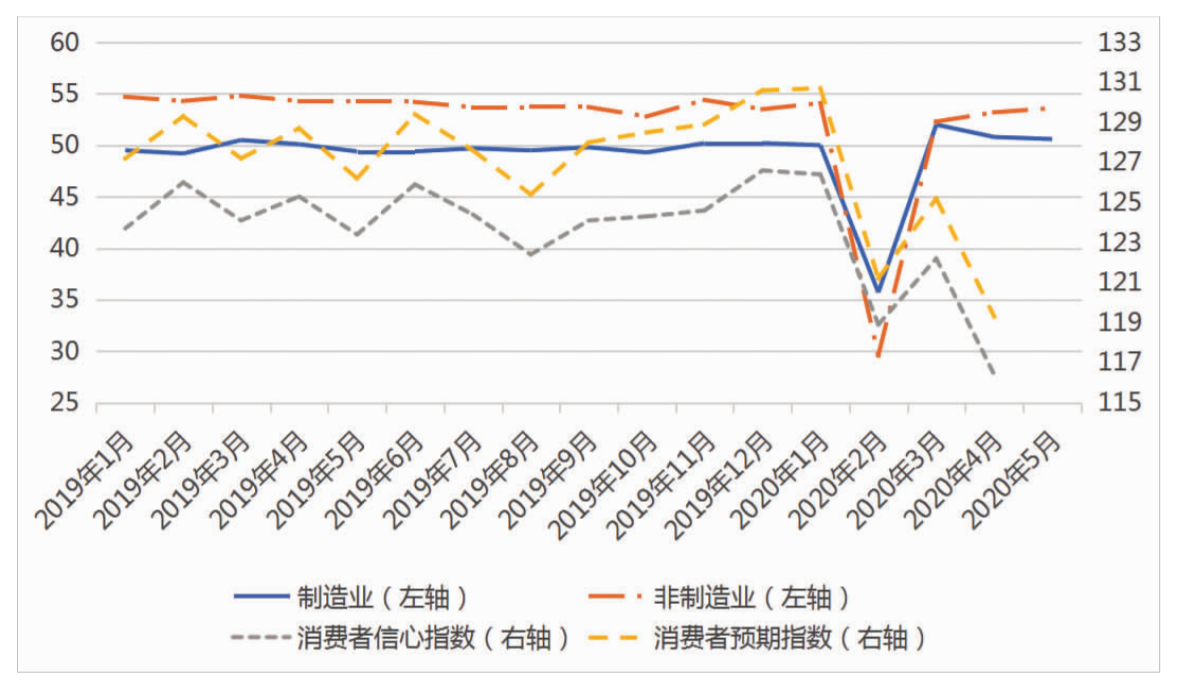
\includegraphics[width=.8\textwidth]{figures/A2.png}
	\caption{采购经理人指数, 消费者预期指数变化图}
	\label{lssssdddssct}
\end{figure}
		\subsection{股市回归模型的建立与求解}
		针对疫情对股票的影响,本文采用基于序列最小最优化(Sequential Minimal Optimization, SMO)的支持向量回归机(Support Vactor Regression, SVR)对股票进行预测,其模型后文简称SMO-SVR。SVR的基本思想是寻找一个最优分类而使得所有训练样本离该最优分类面的误差最小。参考 Kate Childs 等 人的文章\upcite{5},建立出多维传染病决策向量与经济股市之间的 SMO-SVR 模型。
		\subsubsection{支持向量机回归}
		给定训练样本$D=\left\{\left(x_{1}, y_{1}\right),\left(x_{1}, y_{1}\right), \ldots \ldots,\left(x_{m}, y_{m}\right)\right\}
		$,其中$x_i$为特征向量,本文取发病人数、死亡人数、治愈人数和股市平滑值对股价$y_i$进行预测。对于SVR问题可形式化为
				\begin{gather}
\min _{w, b} \frac{1}{2}\|w\|^{2}+C \sum_{i=1}^{m} l_{\epsilon}\left(f\left(x_{i}\right), y_{i}\right),
		\end{gather}
		其中C为正则化常数,lϵ是不敏感损失(insensitive loss)函数:
				\begin{gather*}
l_{\epsilon}(z)=\left\{\begin{array}{cc}
0, & |z| \leq \epsilon ,\\
|z|-\epsilon, & \text {其他}.
\end{array}\right.
\end{gather*}

 由间隔带两侧的松弛程度可以不同,引入松弛变量$\varepsilon_i\geq 0$,其中$\varepsilon_i$对应于的数据点。考虑松弛变量后每个数据点x(i)位于两侧条件为:
 				\begin{gather*}
-\varepsilon-\hat{\xi}_{i} \leq y^{(i)}-f\left(x^{(i)}\right) \leq \varepsilon+\xi_{i} .
 \end{gather*}
 
         因此SVR回归加入松弛因子的误差函数和限制条件可以写为:
  				\begin{gather}
\begin{aligned}
&\min _{w, b} \frac{1}{2}\|w\|_{2}^{2}+C \sum_{i=1}^{m}\left(\hat{\xi}_{i}+\xi_{i}\right),\\
&\text { st. }-\varepsilon-\hat{\xi}_{i} \leq y^{(i)}-f\left(x^{(i)}\right) \leq \varepsilon+\xi,\\
&\xi_{i} \geq 0, \hat{\xi}_{i} \geq 0, i=1,2, \ldots, m.
\end{aligned}
 \end{gather}
 		\subsubsection{序列最小最优化}
 		SMO是一种启发式算法,该算法并不直接求解对偶问题,而是从K-T条件入手,如果所有变量的  解$a^*$都满足此最优化问题的K-T条件,那么这个最优化问题的解就得到了,因为K条件是该最优化 问题的充分必要条件。其SMO算法描述如下
 		
 		\begin{itemize}                                             
 			\item [\textbf{step1.}] 初始化解集$x^{(0)}=0$,令松弛变量$\varepsilon_i= 0$,偏置$k=0$。
 			\item [\textbf{step2.}]选取优化变量$x_1^{(k)},x_2^{(k)}$,解析求解两个变量的最优化问题,求得最优解$x_1^{(k+1)},x_2^{(k+1)}$,更新$x$为$x^{(k+1)}$。
 			\item [\textbf{step3.}] 若在精度ε范围内满足停机条件:
 			  				\begin{gather}
\begin{array}{c}
\sum_{i=1}^{n} x_{i} y_{i}=0, \\
0 \leq \alpha_{i} \leq C, \quad i=1,2, \ldots, n ,\\
x_{i}=0 \Leftrightarrow y_{i} g\left(x_{i}\right) \geq 1 ,\\
0<x_{i}<C \Leftrightarrow y_{i} g\left(x_{i}\right)=1 ,\\
x_{i}=C \Leftrightarrow y_{i} g\left(x_{i}\right) \leq 1,
\end{array}
 			\end{gather}其中$g\left(x_{i}\right)=\sum_{j=1}^{n} \alpha_{j} y_{j} K\left(x_{i}, x_{j}\right)+b
 			$,则转\textbf{step4},否则令$k=k+1$,执行\textbf{step2}
 			\item [\textbf{step4.}] 取解集$x^*=x^{(k+1)}$为最终预测值。
 		\end{itemize}
 		
        \subsection{实验结果及分析}
        
        当中国大陆逐步开始复工复产时,国外疫情开始恶化。 由于疫情爆发等原因,美股在 3 月份四次熔断,对我国的股市造成了不小冲击,沪深 300 指数经历了剧烈的下跌,成交额和融资交易量都呈现下降的态势。 这是在国外疫情形
        势恶化和国内实体经济遭受冲击的共同作用下形成的。下图是疫情对我国股市的影响。
        \begin{figure}[H]
        	\centering
        	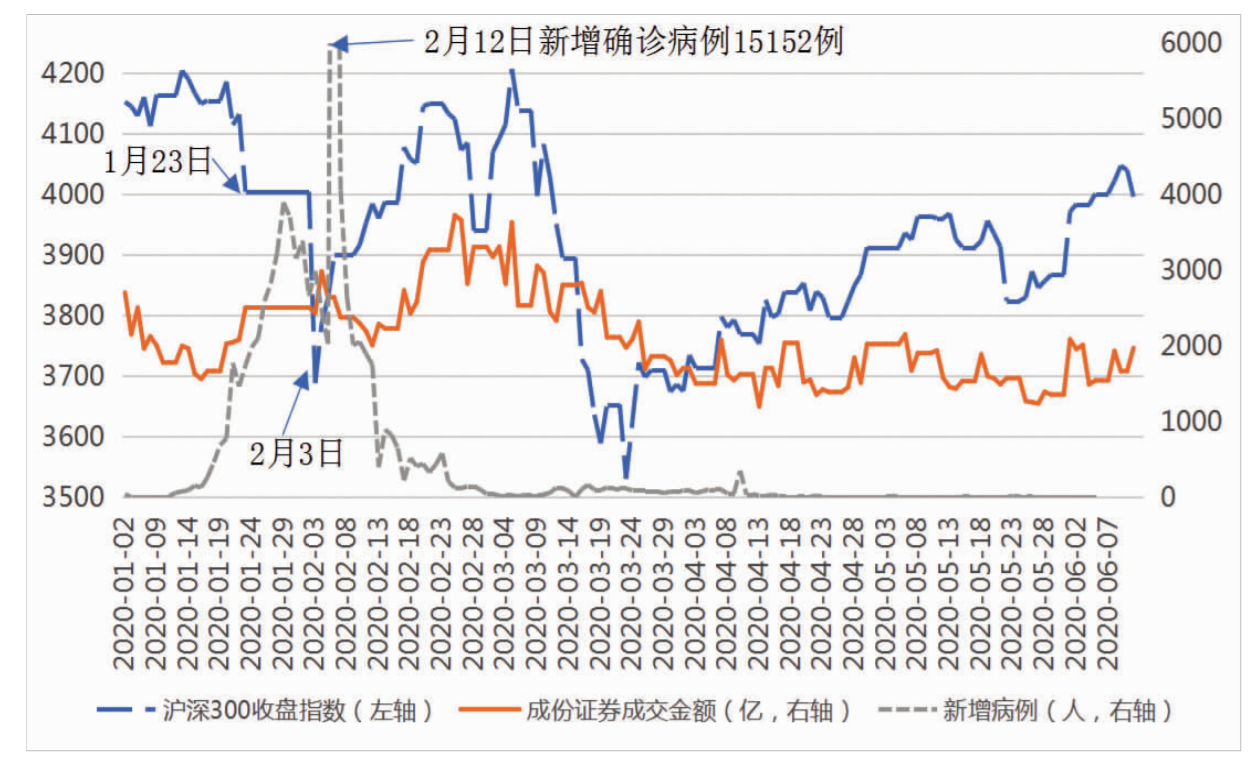
\includegraphics[width=.8\textwidth]{figures/A6.png}
        	\caption{沪深 300 指数与全国新冠肺炎
        		新增感染人数走势对照图}
        \end{figure}
        
        
       就于国外经济体美国而言,本节以苹果的股票价格2020年1月22日至2020年7月20日为例(代码AAPL)进行分析,并对八月股市走向做预测。对于AAPL,今年行情如图\ref{lssssddsssssdssct}所示,从这里我们可以得到大多数股票之间的分布近似正相关。
   
    \begin{figure}[H]
   	\centering
   	\subfigure[AAPL移动平滑图]{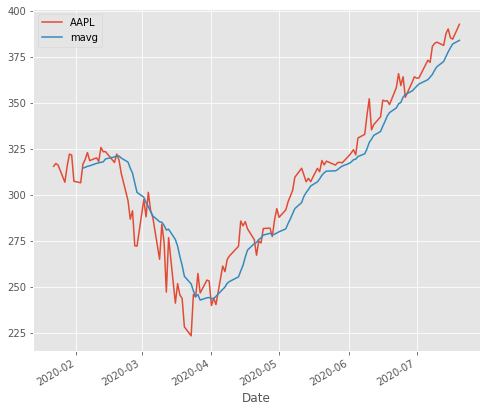
\includegraphics[height=6cm,width=7.5cm]{figures/A3.png}}
   	\subfigure[竞争股票间相关程度]{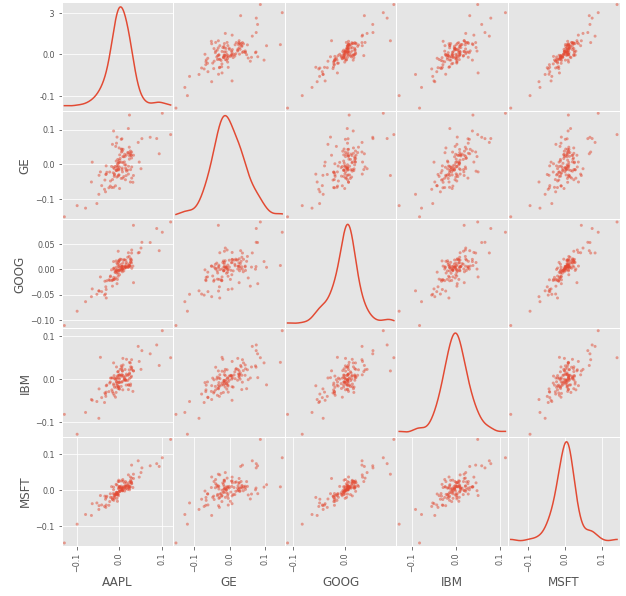
\includegraphics[height=6cm,width=7.5cm]{figures/A4.png}}
   	\caption{疫情条件下,AAPL股市走向与同行业竞争对比}        	\label{lssssddsssssdssct}
   \end{figure}

通过建立的 SVR 模型,首先以美国疫情条件下每天的发病人数,死亡人数,治愈人数和股市平滑值作为模型的输入变量,然后对苹果股价闭盘股市八月份序列最小优化支持向量回归预测,最终得到预测结果:
           \begin{figure}[H]
   	\centering
   	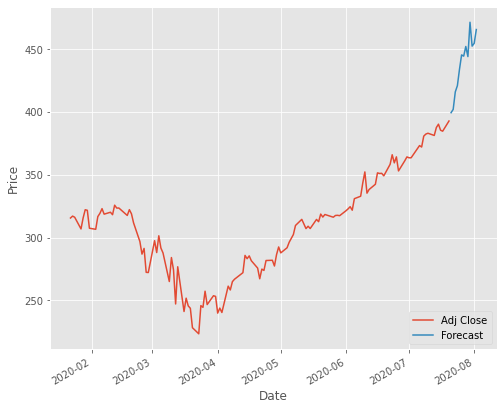
\includegraphics[width=.8\textwidth]{figures/A5.png}
   	\caption{AAPL八月股价预测图}
   \end{figure}

模型分析结果表明股票价格与传染病人数是成负相关,这与世界各地经济与传染病实际情况实相符的。经济衰退不会持续太久,然后就会复苏。因此,我们可以在经济低迷时买进股票,在经济好转时卖出。 其中在五月初阶段,传染病人数每减少200人左右,股价将上升10\$左右。通过对预测结果从均方根误差、平均相对误差绝对值和纳什效率系数三个方面进行验证模型,发现预测误差均接近于5\%,说明了模型的预测效果比较精准、可信度高。

	
    \section{总结与疫情防控建议}
   \noindent
\textbf{尊敬的中国政府公共卫生管理部门:}

针对本次新冠病毒肺炎疫情的发展, 我们提出了一类基于时滞动力学系统的传染病动力学模型。通过该模型,我们不仅反演出了各地的传染率和隔离率,而且有效地预测了各地的疫情发展趋势。数值模拟显示在现有防控力度不放松的情况下,疫情能在较短时间内得到控制并逐步结束。

分析居家令(stay-at-home\ policy)和就地避难令(shelter-in-place\ policy)的防疫效应前,需要根据我们模型的种类,从量化层面理解防疫的最终目的。我们建立的DSEIR动力学模型满足总人群数守恒的假设,因此防疫抗疫的本质是\textbf{降低潜伏者和感染者的占比,提高易感者的占比},在经过一个较长的周期后最终实现感染者清零。

控制其他参数不变,对弱势群体易感者建立的DSEIR模型中的微分方程中,居家令的实施限制了易感者的人口流动,降低了易感人群在随机均匀混合人群中的占比,即有效降低了方程中的有效接触系数$\rho$。这个效应在潜伏者、隔离潜伏者和隔离易感者的控制方程中得到体现,在其他参数不变的情况下有效减缓了这三者的增速。根据模型,因为感染者增速与易感者转化的速率成正比,实施居家令的代价是感染者增速会随着易感者增多而加快,但由于初始状态下易感者人群数目主要体现下降的趋势,执行严格居家令措施将使得疫情高峰于\textbf{30天后}到来。最高感染人数将分别达到\textbf{2万人/60万人},是原始数据的0.7倍。死亡人数将达到\textbf{8百/7万人},是原始数据的0.6倍。即若及时管控严格将使得疫情损失大幅度降低。\textbf{实施居家令可以有效阻止疫情扩散,降低易感人群患病风险}。

此外,\textbf{就地避难令的提出对防疫抗疫也具有深刻意义}。若不实施就地避难令,假设考虑甲乙两地的混合均匀迁入迁出,甲地向乙地单项流动,其中甲是高风险区域,乙是低风险区域,两地区的总人群数目不变。对甲乙两地的总人群,根据改进的SEIR模型,由于人口流动能力增强,接触率$\alpha$增大,与居家令模型效应相反,增大防疫难度。

最后,\textbf{及时的严格隔离措施对减缓疫情也具有重要意义}。以湖北省数据预测曲线可知,推后5日执行严格隔离措施将使得疫情高峰于\textbf{50天后}到来。最高感染人数将分别达到\textbf{5万人/120万人},是原始数据的\textbf{两倍}左右。死亡人数将达到\textbf{3千/14万人},是原始数据\textbf{的3倍}。若使严格隔离措施提前3日执行,即使得1月19日前隔离比例为$q=0.2$,之后的隔离比例为$q=0.99$。

对模型进行综合分析后,我们提出以下建议:

\textbf{第一,在取得防疫成果的基础上不放松警惕。}在取得一定防疫成果的基础上,警惕输入病例和复阳病例,及时隔离观察治疗,防止疫情扩散。小范围的扩散依然要采取早隔离早防治的基本措施。疫苗研究方面同样不能松懈。

\textbf{第二,采取严格隔离措施。}本文改进的动力学模型考察了新增的隔离易感者和隔离潜伏者对疫情走势的综合效应。结果显示尽早执行隔离措施和医学观察可让感染人数和死亡人数减少$30\%$和$40\%$。及时的隔离和严格的医学观察措施可以极大减少疫情损失。

\textbf{第三,以命运共同体的视角对待疫情对全人类的考验。}武汉疫情爆发后,中央采取了举国上下支援武汉、省市对口支援、军队支持等抗疫措施,检测试剂、口罩等补给促进了人群清晰化,火神山、雷神山医院最大程度上为住院患者的治疗提供了帮助,降低了死亡率。在通过付出极大代价钻研出可行的中国方案后,贵机构可以向国际组织反馈防疫抗疫过程中的信息,必要时提供人员、技术、物资等支持。

以上是我们对本文新冠病毒传播模型的分析与提出的建议,愿贵机构考虑。期待在不久的未来,通过人们的共同努力,新冠疫情带来的瘟疫危机能彻底得到解决。


 
  	\section{模型的评价}
		\subsection{模型的优点}
			\begin{itemize}                                             
			\item [(1)]结合了新冠病毒的实际特点改进了SEIR模型,且使用免疫差分进化算法估计参数,使得预测模型更贴近于本次疫情的实际情况。
			\item [(2)]通过序列最小优化算法作为样本的训练算法,进而建立序列最小优化支持向量回归模型,从而减小算法复杂度,提高算法的求解速度。
			\end{itemize}
		\subsection{模型的缺点}
在人群流动分析时,动态DSEIR模型需要基于总人群守恒划分人群仓库,做出严格的模型假设,与实际情况有一定的差别。

  
 
%	\newpage	%换页符
	%%参考文献
	%\begin{thebibliography}{9}%宽度9
	% \setlength{\itemsep}{-2mm}
	\nocite{*}		%排版未引用的参考文献
	\begin{thebibliography}{9}%宽度9
		\bibitem{1}Berger D W, Herkenhoff K F, Mongey S. An seir infectious disease model with testing and conditional quarantine[R]. National Bureau of Economic Research, 2020.
	\bibitem{2}Pandey G, Chaudhary P, Gupta R, et al. SEIR and Regression Model based COVID-19 outbreak predictions in India[J]. arXiv preprint arXiv:2004.00958, 2020.
	\bibitem{3}Hou C, Chen J, Zhou Y, et al. The effectiveness of quarantine of Wuhan city against the Corona Virus Disease 2019 (COVID‐19): A well‐mixed SEIR model analysis[J]. Journal of medical virology, 2020.
	\bibitem{4}陈友鹏, 陈璟华. 基于鲸鱼优化参数的最小二乘支持向量机短期负荷预测方法[J]. 计算机工程, 2019, 37(03): 75-81.
	\bibitem{5}Childs K, Cannon M, Davis C, et al. Reply to:“Is resistance to direct-acting antivirals in sub-Saharan Africa a threat to HCV elimination? Recommendations for action”[J]. Journal of Hepatology, 2020, 72(3): 585-586.
	\bibitem{6}周晓剑, 马义中, 朱嘉钢, 等. 求解非半正定核 Huber-支持向量回归机问题的序列最小最优化算法[J]. 控制理论与应用, 2017, 27(9): 1178-1184.
	\end{thebibliography}

	\newpage
	%附录
	\appendix %%附录
	\section{问题一代码}
		\subsection*{动力学模型--python源代码}
			\begin{lstlisting}[language=python]
			from scipy.optimize import dual_annealing, minimize
			from sklearn.metrics import r2_score
			from collections import namedtuple
			from matplotlib import pyplot as plt
			
			SEIR_PARAM = namedtuple('SEIRparm', ['alpha', 'beta', 'theta'])
			q = 0.000 # 隔离比例
			lamada = 1/14
			sigma = 1/7
			deltaI=0.13
			deltaq=0.13
			d = 2.7*(10**(-4)) #病死率
			gammaI=0.007  #感染者的恢复率
			gammaH=0.014
			
			class SEIR(object):
			def __init__(self, P=None):
			self.P = P
			
			def _forward(self, S, E, I, Sq, Eq, H, D, C, param, max_iter):
			alpha, beta, theta = param
			est = dp.Table(columns=['S', 'E', 'I', 'Sq', 'Eq', 'H', 'D', 'C'])
			for t in range(max_iter):
			rou = S/(S+E+I+C)
			S_ = S - alpha*rou*(beta+q*(1-beta))*(I+theta*E) + lamada*Sq
			# S_ = S - alpha*theta*E - alpha*rou*(beta+q*(1-beta))*I + lamada*Sq
			E_ = E + rou*alpha*beta*(1-q)*(I+theta*E) - sigma*E
			I_ = I + sigma*E - (deltaI+d+gammaI)*I
			Sq_ = Sq + rou*alpha*q*(1-beta)*(I+theta*E) - lamada*Sq
			Eq_ = Eq + rou*alpha*beta*q*(I+theta*E) - deltaq*Eq
			H_ = H + deltaI*I + deltaq*Eq - (d+gammaH)*H
			C_ = C + gammaI*I + gammaH*H
			D_ = D + d*(H+I)
			S, E, I, Sq, Eq, H, D, C = S_, E_, I_, Sq_, Eq_, H_, D_, C_
			est.append_row([S, E, I, Sq, Eq, H, D, C])
			return est
			
			def _loss(self, obs, est):
			assert len(obs) == len(est)
			loss = ((np.log2(obs + 1) - np.log2(est + 1)) ** 2).sum() 
			# loss = (np.abs(1-est['I']/obs['I'])+np.abs(1-est['D']/obs['D'])
			#                 +np.abs(1-est['C']/obs['C'])).sum()
			# print(est)
			self.lossing.append(loss)
			return loss
			
			def _optimize(self, param, s, e, i, sq, se, h, d, c, obs):
			est = self._forward(s, e, i, sq, se, h, d, c, param, len(obs))
			return self._loss(obs, est['I', 'D', 'C'].toarray())
			
			def fit(self, initS, initE, initI, initSq, initEq, initH, initD, initC, Y):
			self.lossing = []
			args = (initS, initE, initI, initSq, initEq, initH, initD, initC, Y['确诊', '死亡', '治愈'].toarray())
			param = [(0, 1),] * 3
			# result = minimize(self._optimize, [random()] * 5, args=args, bounds=param)['x']
			result = dual_annealing(self._optimize, param, args=args, seed=30, maxiter=50)['x']
			self.P = SEIR_PARAM(*result)
			
			def score(self, initS, initE, initI, initSq, initEq, initH, initD, initC, Y, plot=False):
			est = self._forward(initS, initE, initI, initSq, initEq, initH, initD, initC, self.P, len(Y))['I', 'D', 'C']
			loss = self._loss(Y['确诊', '死亡', '治愈'].toarray(), est.toarray())
			est.columns = ['确诊', '死亡', '治愈']
			r1 = r2_score(Y['治愈'], est['治愈'])
			r2 = r2_score(Y['死亡'], est['死亡'])
			r3 = r2_score(Y['确诊'], est['确诊'])
			if plot:
			self.plot_predict(Y, est)
			print(' - 平均潜伏期为:%.2f天' % (1.0 / self.P.beta))
			# print(' - 病毒再生基数:%.2f' % (self.P.alpha1 / self.P.beta + (self.P.alpha2 / self.P.sigma + self.P.alpha2 / self.P.gamma)/ 2))
			print(' - 确诊R2:%.4f' % r3)
			print(' - 死亡R2:%.4f' % r2)
			print(' - 治愈R2:%.4f' % r1)
			print(' - 模型R2:%.4f' % ((r1 + r2 + r3) / 3))
			print(' - 模型总误差:%.4f' % loss)
			return loss, (r1 + r2 + r3) / 3
			
			def plot_error(self):
			# plt.rcParams['font.sans-serif'] = ['SimHei']
			plt.plot(self.lossing, label=u'正确率')
			plt.legend()
			plt.show()
			
			def plot_predict(self, obs, est):
			for label, color in zip(obs.keys(), ['red', 'black', 'green']):
			# plt.rcParams['font.sans-serif'] = ['SimHei']
			plt.plot(obs[label], color=color)
			print(label)
			plt.plot(est[label], color=color, alpha=0.7)
			plt.legend()
			plt.show()
			
			def predict(self, initS, initE, initI, initSq, initEq, initH, initD, initC, T):
			
			return self._forward(initS, initE, initI, initSq, initEq, initH, initD, initC, self.P, T)
			
			
			train = data['患病','死亡','治愈']
			train.columns = ['确诊', '死亡', '治愈']
			train.accumulate(inplace=True)
			
			S = 900000000
			I = 1
			Sq = 200000
			Eq = 420000
			H = 20
			D = 0
			C = 0
			
			def searchBestParam(seir, S, I, Sq, Eq, H, D, C):
			min_loss, max_r2, best_param, likeli_potential = float('inf'),0.0, None, 0
			for potential in range(0, 500, 25):
			seir.fit(S, potential, I, Sq, Eq, H, D, C, train)
			loss, r2 = seir.score(S, potential, I, Sq, Eq, H, D, C, Y=train)
			print(loss,r2)
			if loss < min_loss: # and r2 > max_r2:
			print('潜在患者:%.4f | R2:%.4f | 误差: %.6f' % (potential, r2, loss))
			min_loss, max_r2, best_param, likeli_potential = loss, r2, seir.P, potential
			seir.P = best_param
			print(seir.P, likeli_potential)
			seir.score(S, likeli_potential, I, Sq, Eq, H, D, C, Y=train, plot=True)
			return seir, likeli_potential
			
			seir, potentials = searchBestParam(SEIR(), S, I, Sq, Eq, H, D, C)
			
			
			def forcast(seir, T):
			predict = seir.predict(S, potentials, I, Sq, Eq, H, D, C, T)
			plt.plot(train['确诊'], label='确诊(真实)', color='red')
			plt.plot(train['死亡'], label='死亡(真实)', color='black')
			plt.plot(train['治愈'], label='治愈(真实)', color='green')
			# plt.plot(predict['S'], label='易感(预计)', color='blue', alpha=0.5)
			plt.plot(predict['E'], label='潜伏(预计)', color='orange', alpha=0.5)
			plt.plot(predict['I'], label='确诊(预计)', color='red', alpha=0.5)
			plt.plot(predict['D'], label='死亡(预计)', color='black', alpha=0.5)
			plt.plot(predict['C'], label='治愈(预计)', color='green', alpha=0.5)
			plt.legend()
			plt.show()
			forcast(seir, 30)
			\end{lstlisting}
			
		\subsection*{免疫遗传求解--python源代码}
\begin{lstlisting}[language=python]
# -*- coding: cp936 -*-
import numpy as np
import matplotlib.pyplot as plt
import math
import random

# Rastrigr 函数
def object_function(x):
f = 0
for i in range(0,len(x)):
f = f + (x[i] ** 2 - (10 * math.cos(2 * np.pi * x[i])) + 10)
return f
# 参数
def initpara():
NP = 100   # 种群数量
F = 0.6   # 缩放因子
CR = 0.7   # 交叉概率
generation = 2000   # 遗传代数
len_x = 10
value_up_range = 5.12
value_down_range = -5.12
return NP, F, CR, generation, len_x, value_up_range, value_down_range
# 种群初始化
def initialtion(NP):
np_list = []   # 种群,染色体
for i in range(0,NP):
x_list = []   # 个体,基因
for j in range(0,len_x):
x_list.append(value_down_range + random.random() * (value_up_range - value_down_range))
np_list.append(x_list)
return np_list
# 列表相减
def substract(a_list,b_list):
a = len(a_list)
new_list = []
for i in range(0,a):
new_list.append(a_list[i]-b_list[i])
return new_list
# 列表相加
def add(a_list,b_list):
a = len(a_list)
new_list = []
for i in range(0,a):
new_list.append(a_list[i]+b_list[i])
return new_list
# 列表的数乘
def multiply(a,b_list):
b = len(b_list)
new_list = []
for i in range(0,b):
new_list.append(a * b_list[i])
return new_list
# 变异
def mutation(np_list):
v_list = []
for i in range(0,NP):
r1 = random.randint(0,NP-1)
while r1 == i:
r1 = random.randint(0,NP-1)
r2 = random.randint(0,NP-1)
while r2 == r1 | r2 == i:
r2 = random.randint(0,NP-1)
r3 = random.randint(0,NP-1)
while r3 == r2 | r3 == r1 | r3 == i:
r3 = random.randint(0,NP-1)

v_list.append(add(np_list[r1], multiply(F, substract(np_list[r2],np_list[r3]))))
return v_list
# 交叉
def crossover(np_list,v_list):
u_list = []
for i in range(0,NP):
vv_list = []
for j in range(0,len_x):
if (random.random() <= CR) | (j == random.randint(0,len_x - 1)):
vv_list.append(v_list[i][j])
else:
vv_list.append(np_list[i][j])
u_list.append(vv_list)
return u_list
# 选择
def selection(u_list,np_list):
for i in range(0,NP):
if object_function(u_list[i]) <= object_function(np_list[i]):
np_list[i] = u_list[i]
else:
np_list[i] = np_list[i]
return np_list
# 主函数
NP, F, CR, generation, len_x, value_up_range, value_down_range = initpara()
np_list = initialtion(NP)
min_x = []
min_f = []
xx = []
for i in range(0,NP):
xx.append(object_function(np_list[i]))
min_f.append(min(xx))
min_x.append(np_list[xx.index(min(xx))])
for i in range(0,generation):
v_list = mutation(np_list)
u_list = crossover(np_list,v_list)
np_list = selection(u_list,np_list)
for i in range(0,NP):
xx = []
xx.append(object_function(np_list[i]))
min_f.append(min(xx))
min_x.append(np_list[xx.index(min(xx))])
# 输出
min_ff = min(min_f)
min_xx = min_x[min_f.index(min_ff)]
print('the minimum point is x ')
print(min_xx)
print('the minimum value is y ')
print(min_ff)
# 画图
x_label = np.arange(0,generation+1,1)
plt.plot(x_label, min_f)
plt.xlabel('iteration')
plt.ylabel('fx')
plt.savefig('./iteration-f.png')
plt.show()
\end{lstlisting}
	\section{问题二代码}
\subsection*{SMO-SVR模型--python源代码}
\begin{lstlisting}[language=python]
! pip install pandas_datareader

import pandas as pd
import datetime
import pandas_datareader.data as web
from pandas import Series, DataFrame

start = datetime.datetime(2020, 1, 22)

end = datetime.datetime(2020, 7, 20)

df = web.DataReader("AAPL", 'yahoo', start, end)

df.tail()

import matplotlib.pyplot as plt
from matplotlib import style

# Adjusting the size of matplotlib
close_px = df['Adj Close']
mavg = close_px.rolling(window=10).mean()
import matplotlib as mpl
mpl.rc('figure', figsize=(8, 7))

mpl.__version__

# Adjusting the style of matplotlib

style.use('ggplot')

close_px.plot(label='AAPL')

mavg.plot(label='mavg')

plt.legend()

rets = close_px / close_px.shift(1) - 1

rets.plot(label='return')

dfcomp = web.DataReader(['AAPL', 'GE', 'GOOG', 'IBM', 'MSFT'],'yahoo',start=start,end=end)['Adj Close']

retscomp = dfcomp.pct_change()

corr = retscomp.corr()

plt.scatter(retscomp.AAPL, retscomp.GE)

plt.xlabel('Returns AAPL')

plt.ylabel('Returns GE')

pd.plotting.scatter_matrix(retscomp, diagonal='kde', figsize=(10, 10))

plt.imshow(corr, cmap='hot', interpolation='none')
plt.colorbar()

plt.xticks(range(len(corr)), corr.columns)
plt.yticks(range(len(corr)), corr.columns)

dfreg = df.loc[:,['Adj Close','Volume']]

dfreg['HL_PCT'] = (df['High'] - df['Low']) / df['Close'] * 100.0

dfreg['PCT_change'] = (df['Close'] - df['Open']) / df['Open'] * 100.0

import math
import numpy as np
from sklearn.linear_model import LinearRegression
from sklearn.neighbors import KNeighborsRegressor
from sklearn.linear_model import Ridge
from sklearn.preprocessing import PolynomialFeatures
from sklearn.pipeline import make_pipeline
from sklearn import preprocessing
# Drop missing value
dfreg.fillna(value=-99999, inplace=True)

# We want to separate 1 percent of the data to forecast
forecast_out = int(math.ceil(0.1 * len(dfreg)))

# Separating the label here, we want to predict the AdjClose

forecast_col = 'Adj Close'
dfreg['label'] = dfreg[forecast_col].shift(-forecast_out)

X = np.array(dfreg.drop(['label'], 1))

# Scale the X so that everyone can have the same distribution for linear regression
X = preprocessing.scale(X)

# Finally We want to find Data Series of late X and early X (train) for model generation and evaluation
X_lately = X[-forecast_out:]
X = X[:-forecast_out]

# Separate label and identify it as y
y = np.array(dfreg['label'])
y = y[:-forecast_out]

# Linear regression
clfreg = LinearRegression(n_jobs=-1)
clfreg.fit(X, y)

# Quadratic Regression 2
clfpoly2 = make_pipeline(PolynomialFeatures(2), Ridge())
clfpoly2.fit(X, y)

# Quadratic Regression 3
clfpoly3 = make_pipeline(PolynomialFeatures(3), Ridge())
clfpoly3.fit(X, y)

forecast_set = clfpoly2.predict(X_lately)
dfreg['Forecast'] = np.nan

last_date = dfreg.iloc[-1].name

last_unix = last_date

next_unix = last_unix + datetime.timedelta(days=1)

for i in forecast_set:

next_date = next_unix
next_unix += datetime.timedelta(days=1)
dfreg.loc[next_date] = [np.nan for _ in range(len(dfreg.columns)-1)]+[i]

dfreg['Adj Close'].tail(500).plot()
dfreg['Forecast'].tail(500).plot()
plt.legend(loc=4)
plt.xlabel('Date')
plt.ylabel('Price')
plt.show()
\end{lstlisting}
\end{document}